As part of a collaborative \textit{Arts, Science and Culture} Grant sponsored by the University of Chicago's Institute for Molecular Engineering, Divisions of the Biological and Physical Sciences, the Humanities, and the Office of the Vice President for Research and for National Laboratories, I undertook an artistic collaboration project with MFA student at the Art Institute of Chicago, Keeley Haftner.  The following is the text of our narrative proposal and the outcome images presented in our public talk.

Haftner is a Master of Fine Arts candidate in the Fiber and Material Studies department at the School of the Art Institute of Chicago, a department which focuses on the interdisciplinary study of the meaning and manipulation of materials through processes that involve politics, labour, gender, class and value. After meeting to discuss our specific areas of specialization and interest, however, it quickly became clear that our overlap was far more extensive and generative than general interests in the meaning and outcomes of manipulating material forms. Haftner is interested in value as it relates to materials, particularly the valueless. She transforms those materials into potentially valuable forms by employing a process of partial or complete transformation, which in a large part of her studio practice has involved taking waste plastics and transforming them into 3D printing filament with which to make sculptural multiples. McFadden, too, is fascinated by filament and renewal. In his work he studies how the cell's material properties give it the ability to change its own shape and migrate through its surroundings using its cytoskeletal structuring – essentially a web-like sphere made from biopolymer filaments. He is also is focused on sustainability issues, emphasizing how biological materials can inspire new and sustainable technologies. This back and forth, combined with the link of the metaphorical and physical concept of filament, offers up extremely fertile ground for collaboration.

In terms of the physical manifestation of their collaboration, Haftner and McFaddenhave an overlapping material and technological interest that relates to both of their studies: 3D printing and polymer filament. PLA, or Polylactic Acid, is one of the most commonly used plastics in 3D printing. PLA is a naturally derived synthetic polymer which most additive manufacturers consider environmentally friendly because it purports to be compostable. This is important to many makers, since opinions around the topic of 3D printing can be extreme – articles often portray 3D printing as yet another elite frivolity producing unnecessary consumer garbage. PLA is a waste product from agricultural industry typically recouped from corn and sugar production. It is ‘industrially compostable’, which means exactly what it implies: that on an industrial scale, it can be composted. Industrial composting consists of mounding large-scale piles of organic matter and dirt, allowing these materials to combust and reach high temperatures. These piles are overturned and cycled with large-scale equipment until the matter has broken down entirely and become soil. PLA cannot be composted in backyards, it contaminates recycling streams when lumped in with other plastics, and it has the same (nearly infinite) lifespan as other plastics if it ends up in the landfill, the ocean, or as litter on the ground. These plastics rarely end up where they’re meant to go, but they could, if people knew more.

Not only does the interesting material dilemma of PLA merge McFadden and Haftner’s interests, but it is also rich research-based and metaphorical territory. The moment when industrial composting is in the process of biodegradation is the nexus of their research: Haftner’s macro synthetic materials are broken down at the micro level by McFadden’s microorganisms. The inorganic and the organic merge in a moment of decay that is both creation and destruction. This process takes into account the complexity of life, and starts to incorporate notions of Object Oriented Ontology from philosophy, a theory of the study of existence which purports that inorganic things are just as important and contingent as organic life, as well as poetical notions that gesture toward death and life cycles as they relate to existence in general. Anthropologist Tim Ingold speaks of materials as having their own life and trajectory, stating that the point of creation is simply a moment in time in which the scientist, artist, engineer or architect merely intervenes on material form. Both McFadden and Haftner seek to lend meaning to that intervention, in ways that encourage sustainable insights toward our stewardship of ‘things’ in favour of collective re-examination.

The outcome of this collaboration will take the form of a series of sculptures made from both homemade filament from waste PLA plastics, and perhaps other plastic materials as they become relevant, with the possibility of using the filament extruder as the direct sculptural production site itself to make ‘filament sculpture.’ These filament sculptures could perhaps borrow from both the cytoskeletal forms at the heart of McFadden’s research interests, and the conceptual interests that Haftner has in the idea of filament as a binder, a string, a connector, and an object of potential. The production, presentation, and documentation of both the process of making these sculptural multiples and the resultant multiples themselves will be the focus of this collaboration. The nature of this material investigation leaves plenty of room for unknown discoveries through the generative overlap of the pair’s research and processes. As per the schedule for the work, Haftner and McFadden intend to purchase the new equipment as soon as possible and begin experimenting with materials on the previous model until it arrives. They will visit the compost facility in November, and meet once every two weeks for long sessions from November to May to research, play with materials, and experiment with conceptual and visual forms.





\section{Experiments with plastic filament sculpture}

{\setstretch{1.0}
	\blockquote{ The ship wherein Theseus and the youth of Athens returned from Crete had thirty oars, and was preserved by the Athenians down even to the time of Demetrius Phalereus, for they took away the old planks as they decayed, putting in new and stronger timber in their places, in so much that this ship became a standing example among the philosophers, for the logical question of things that grow; one side holding that the ship remained the same, and the other contending that it was not the same. ---Plutarch's Life of Theseus, as translated by John Dryden }
}

\begin{figure}[h!]
\centering
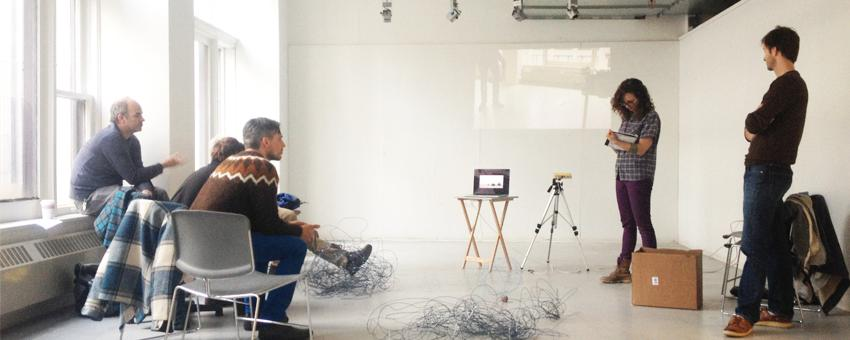
\includegraphics[width=\hsize]{art/collab1.jpg}
\caption{\label{fig:art_2} Feedback session with Art Institute Professors }
\end{figure}

\begin{figure}[h!]
\centering
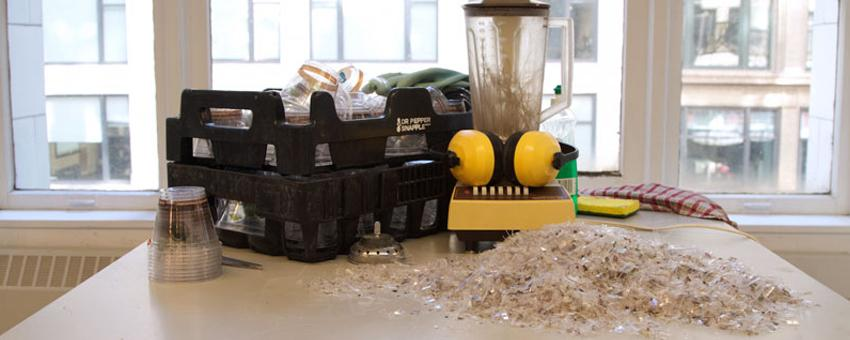
\includegraphics[width=\hsize]{art/shavings.jpg}
\caption{\label{fig:art_1} PLA shavings and blender }
\end{figure}

\begin{figure}[h!]
\centering
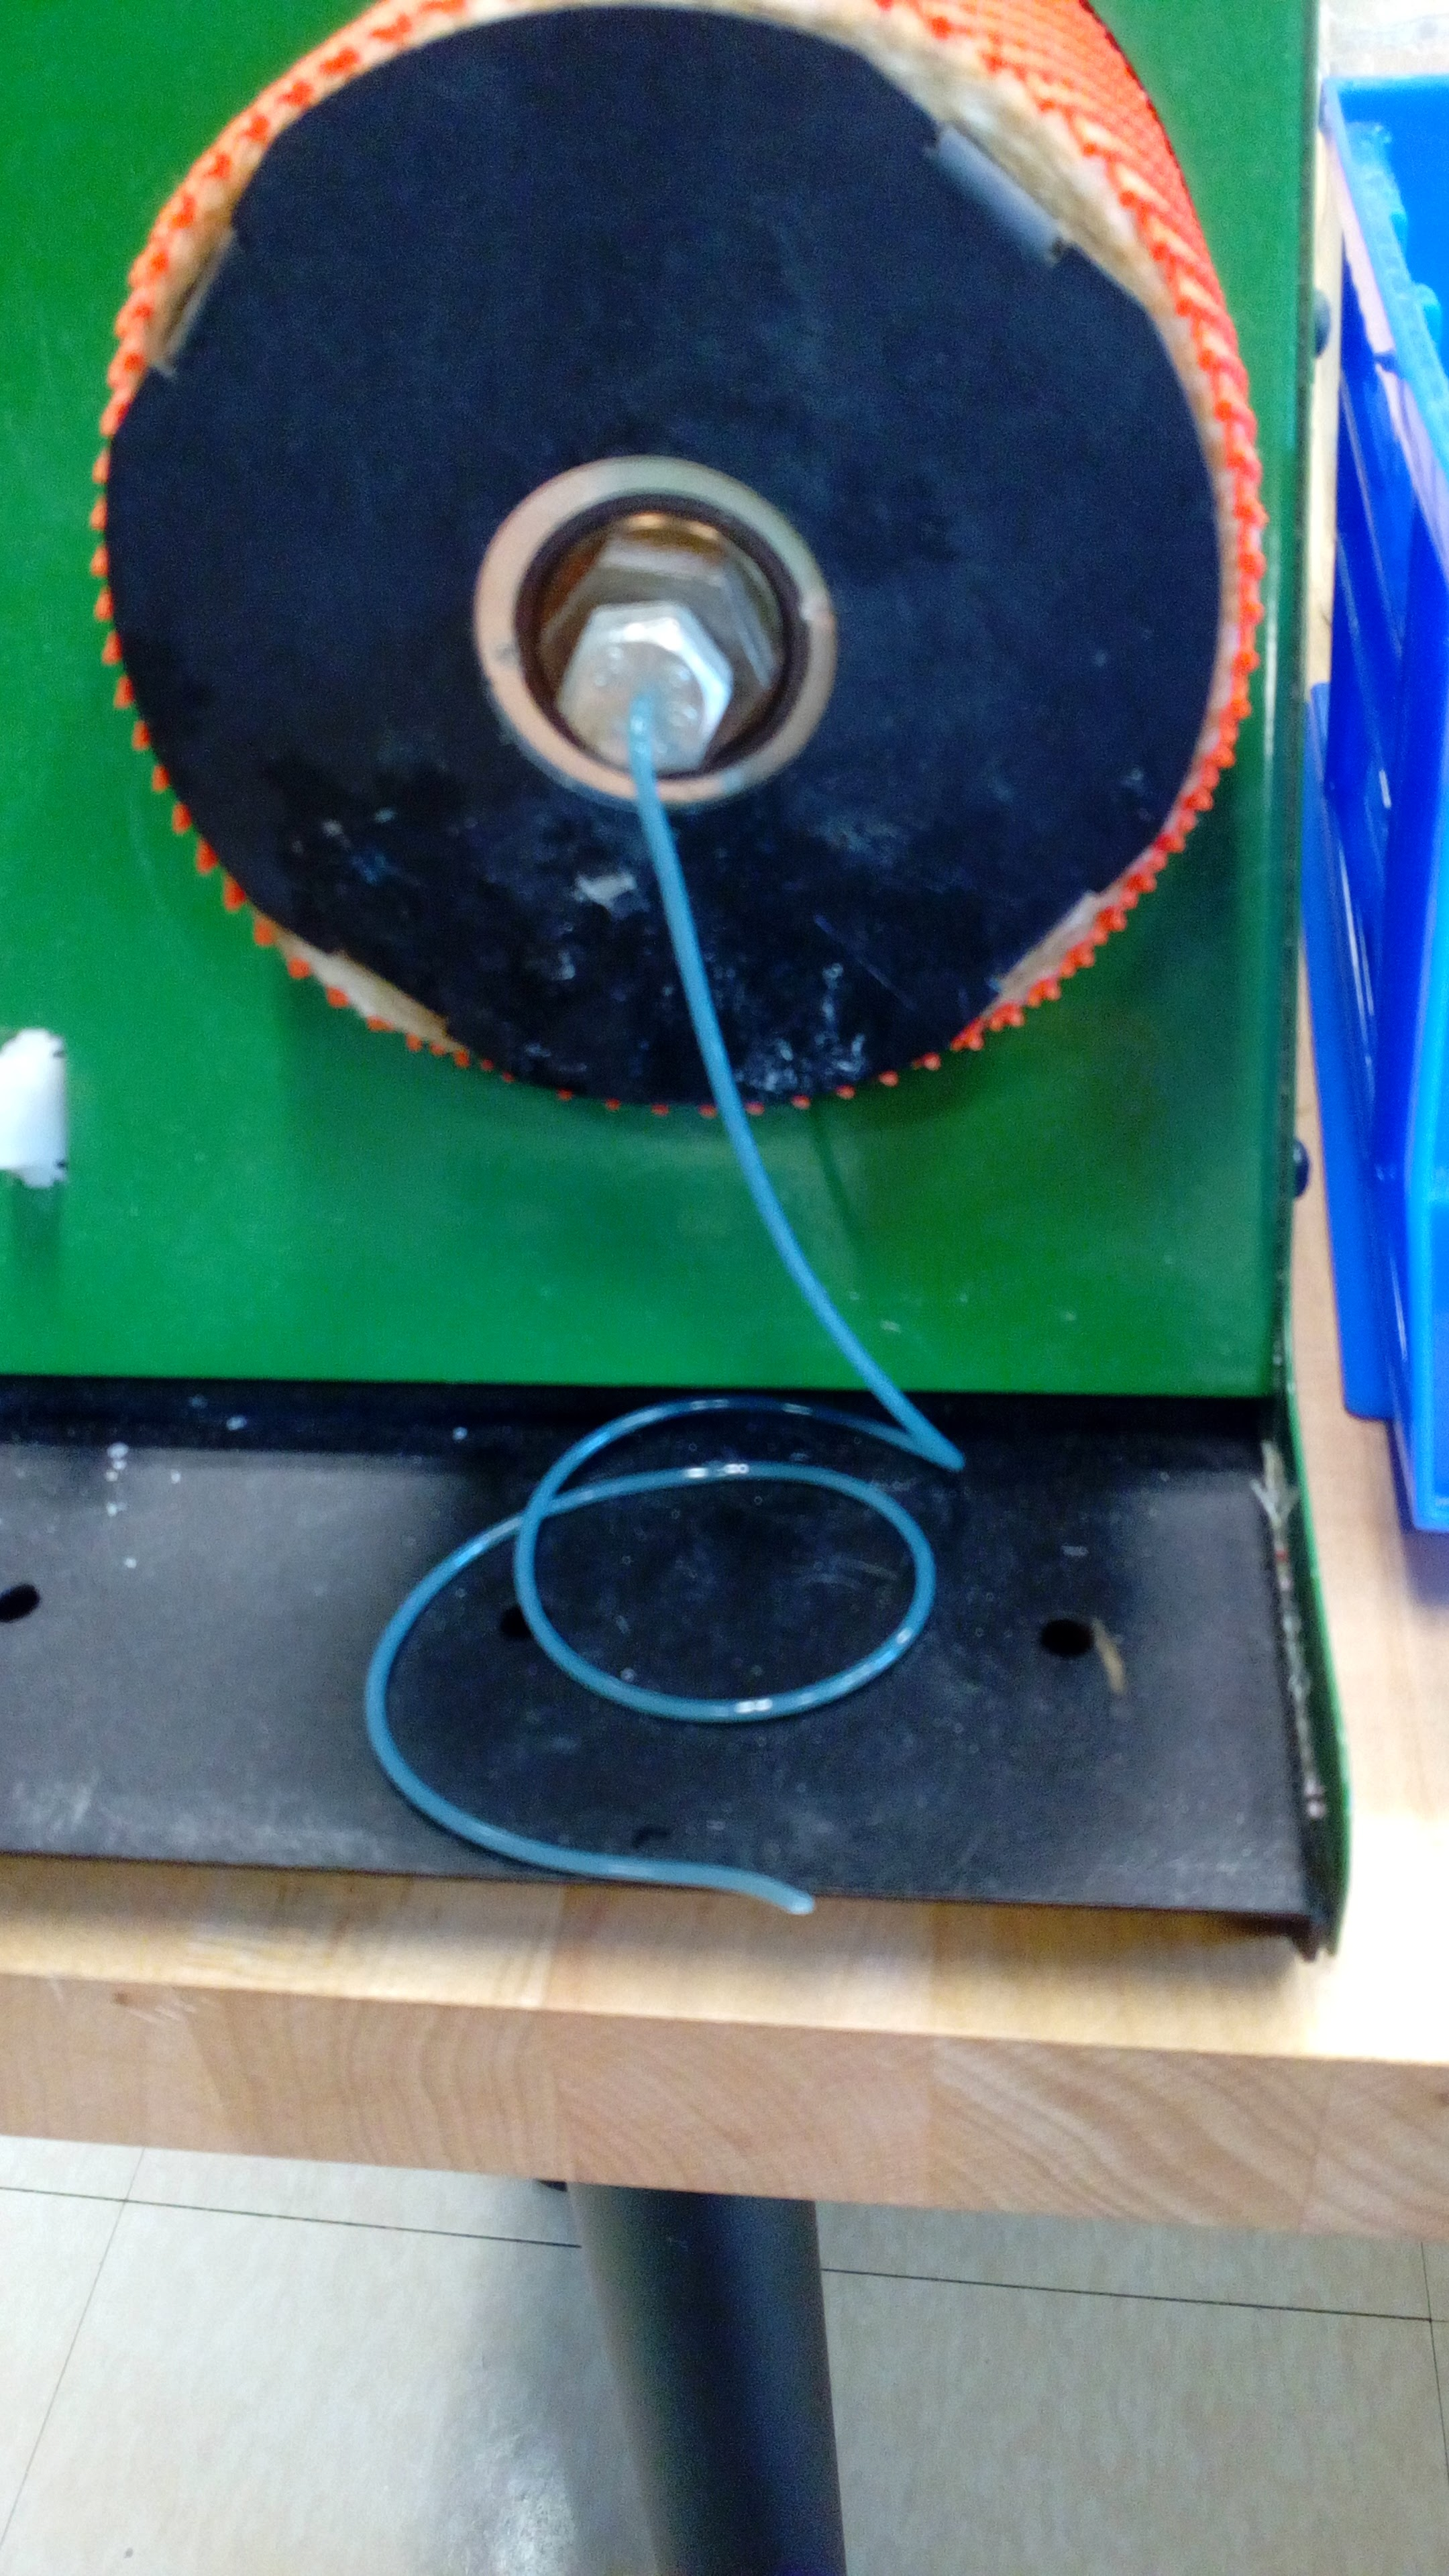
\includegraphics[width=0.5\hsize]{art/IMG_20160801_121017.jpg}
\caption{\label{fig:art_2} Filament extruder }
\end{figure}

\begin{figure}[h!]
\centering
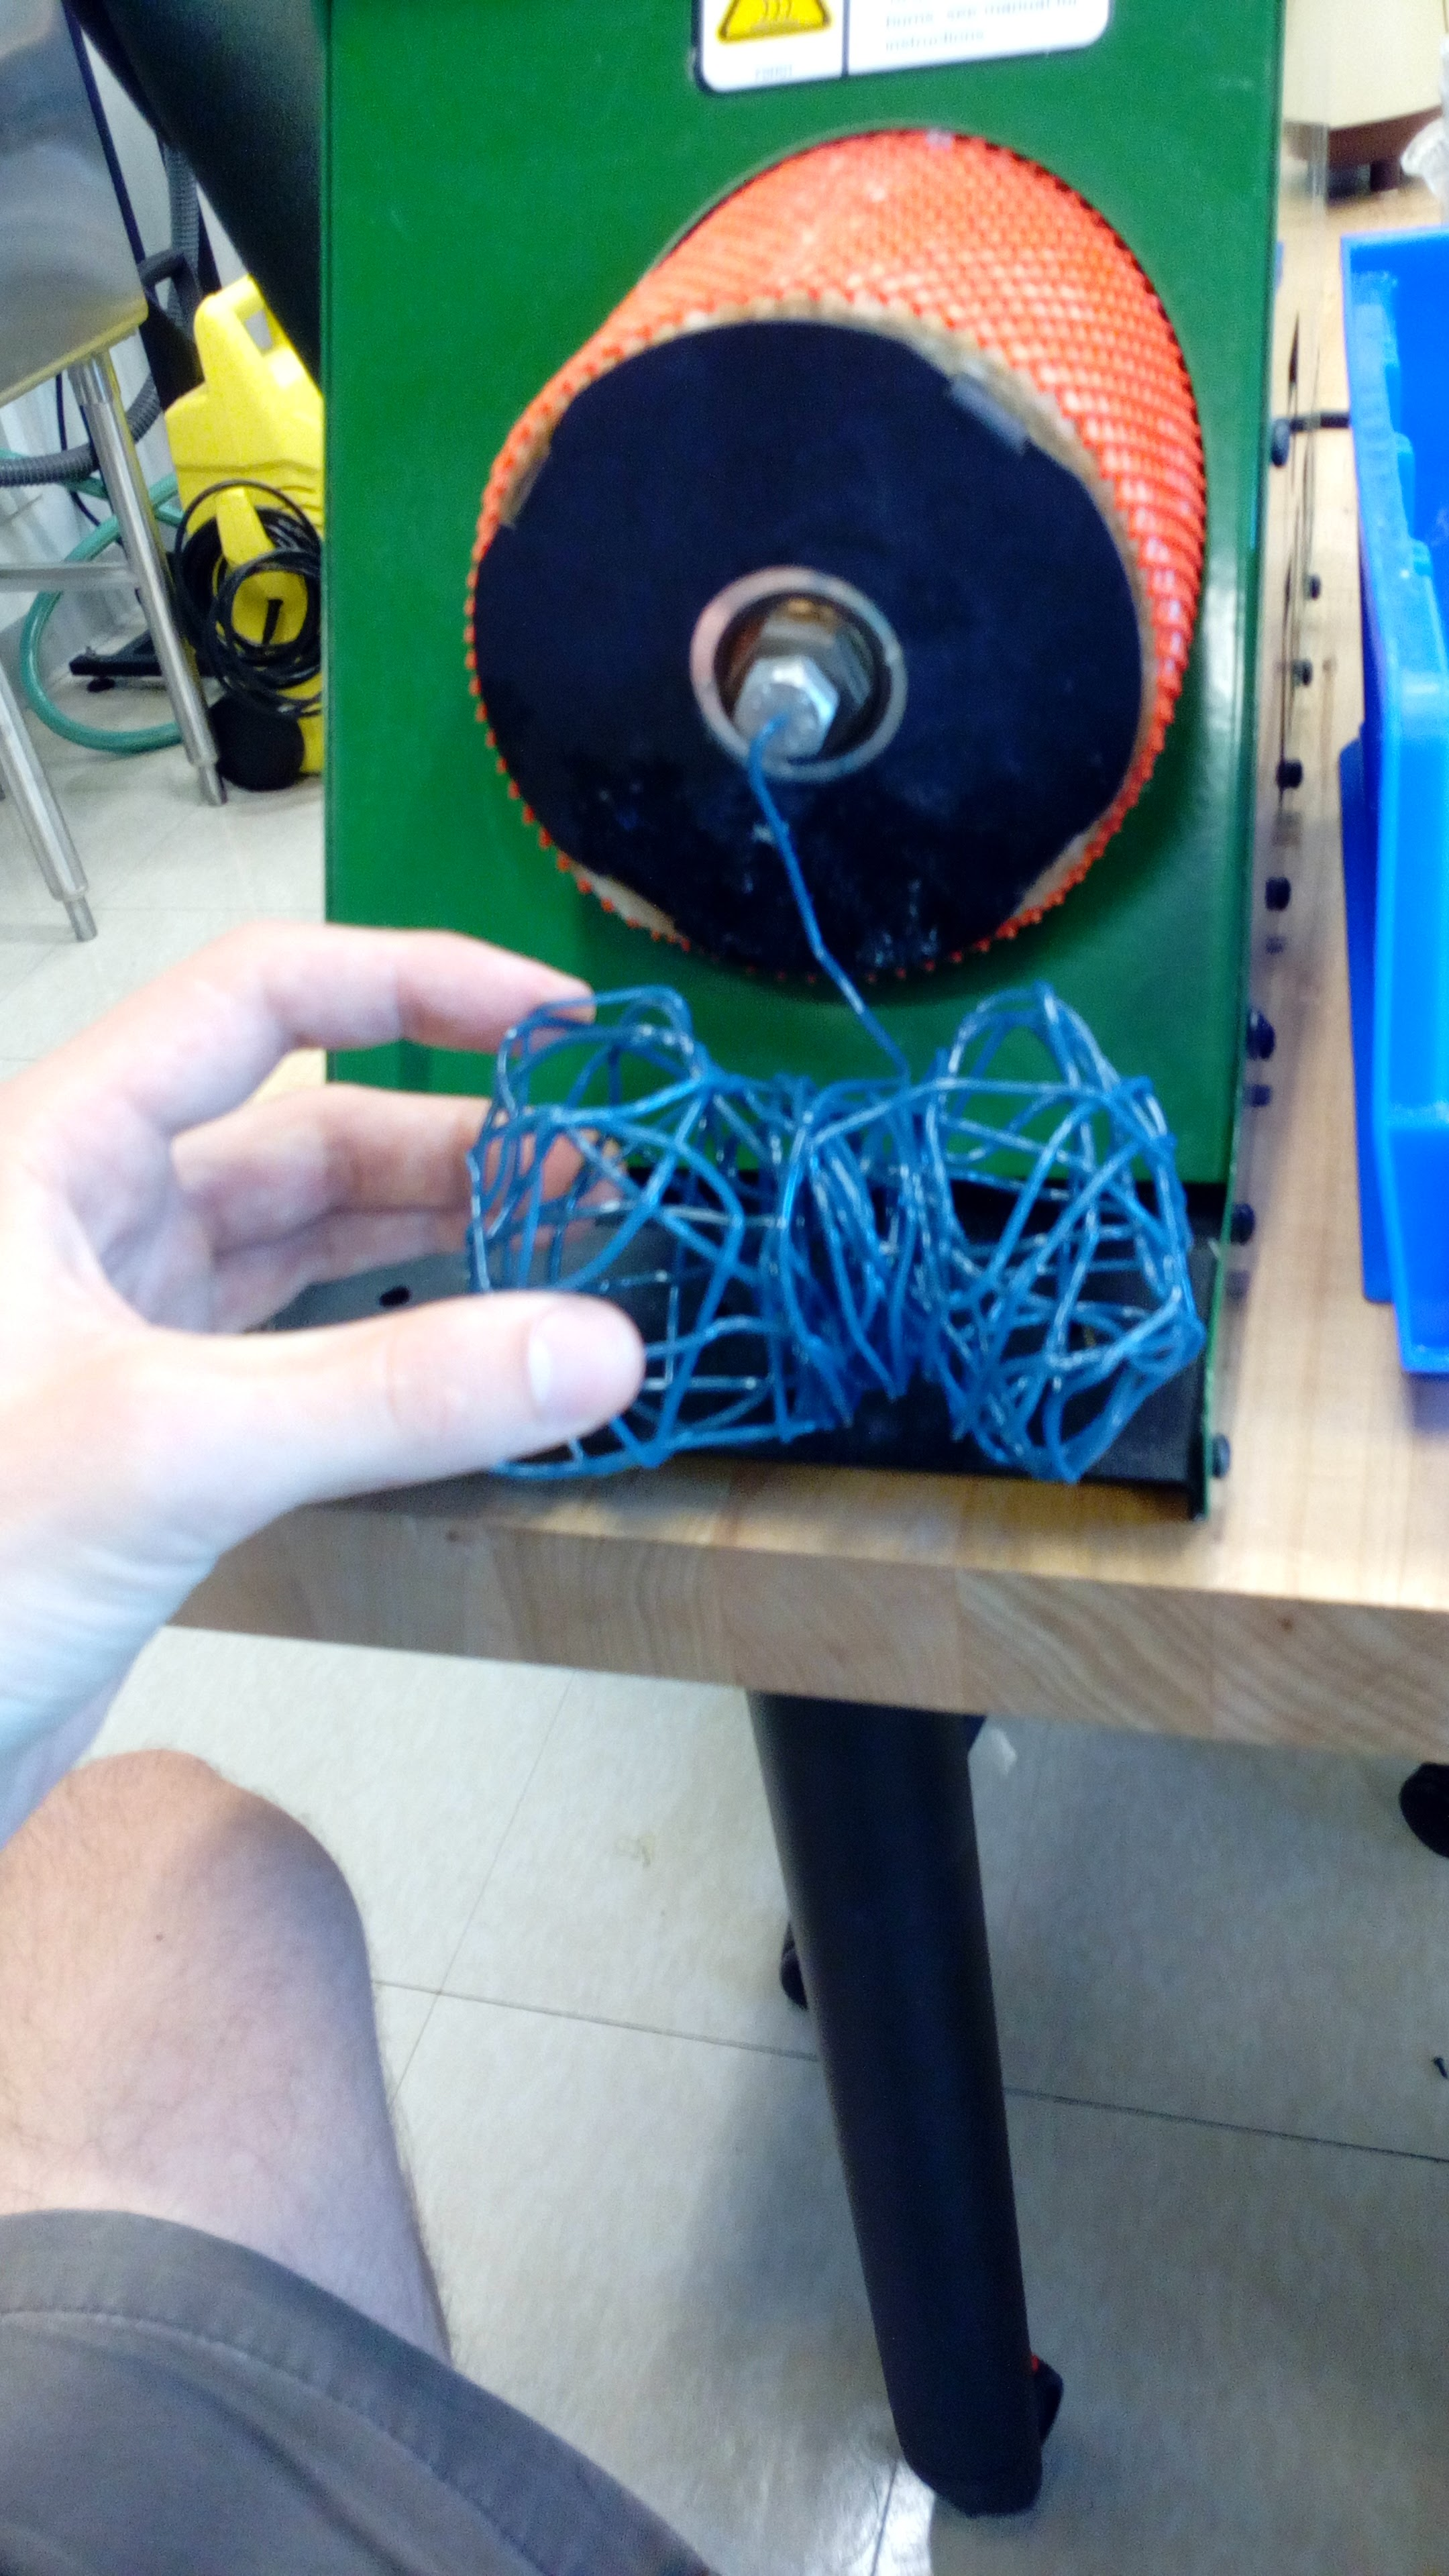
\includegraphics[width=0.5\hsize]{art/IMG_20160801_115125.jpg}
\caption{\label{fig:art_1} Sculpting a dividing cell cytoskeleton }
\end{figure}



\begin{figure}[h!]
\centering
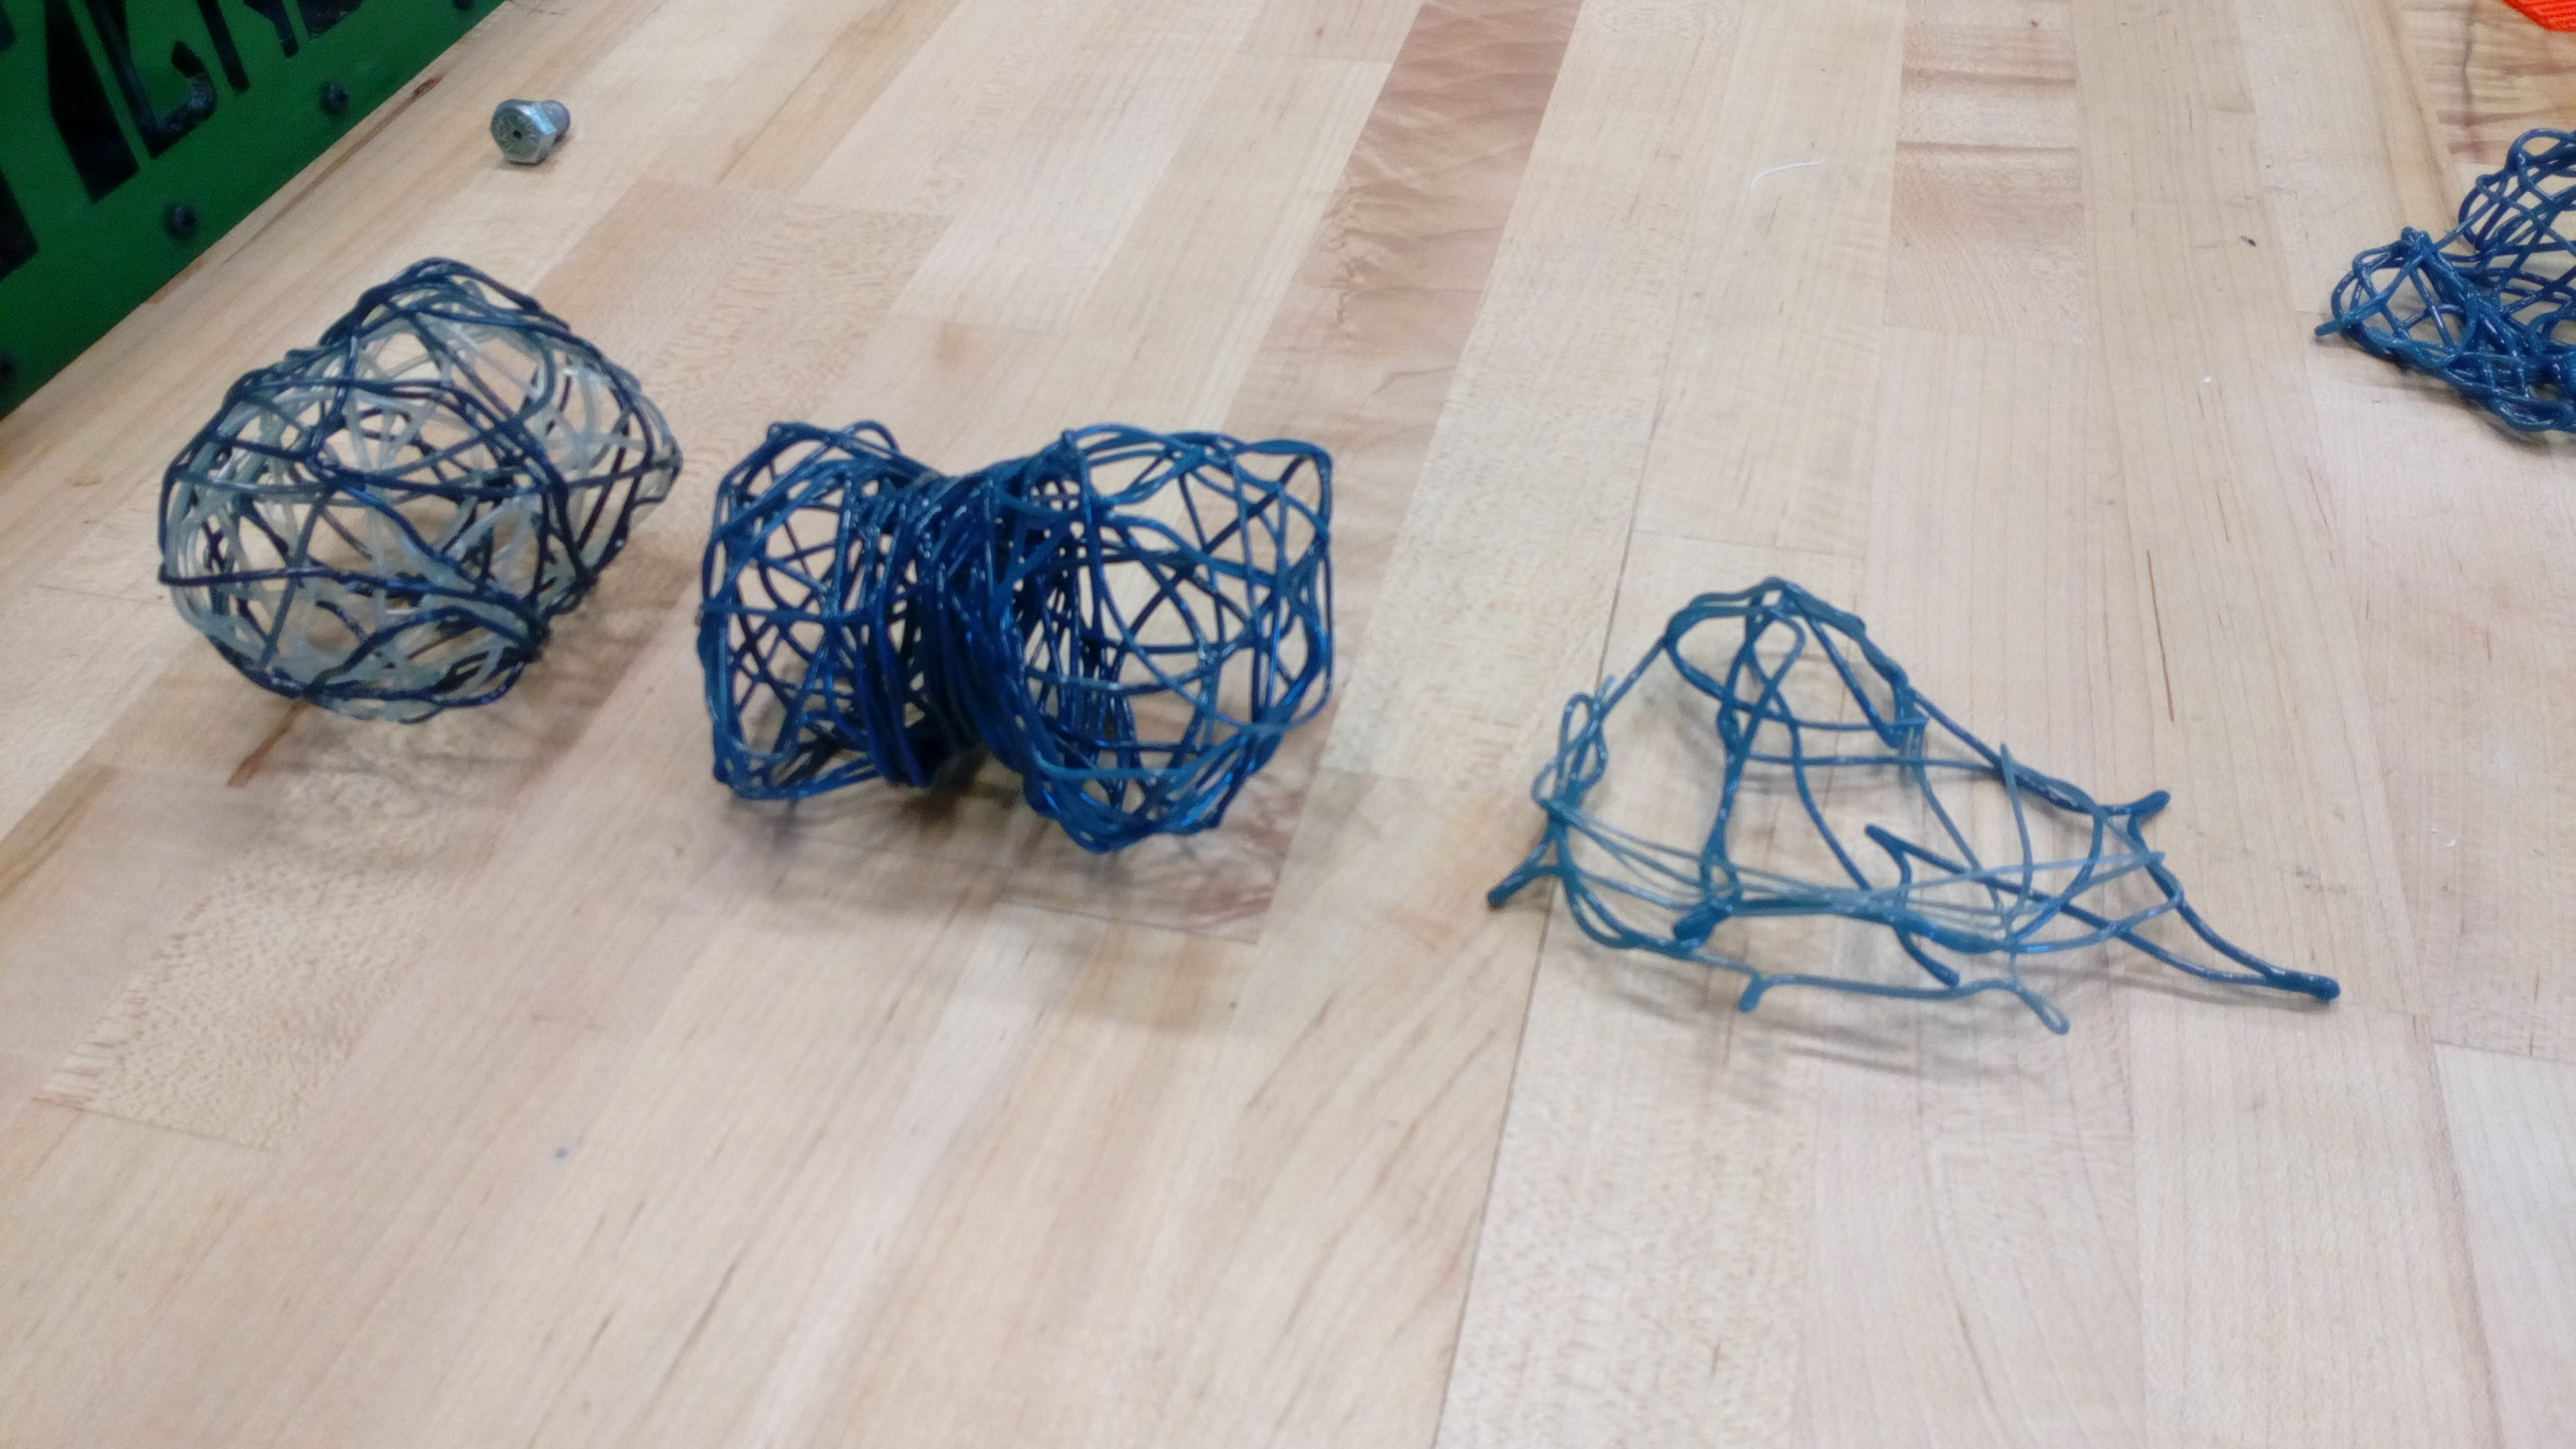
\includegraphics[width=\hsize]{art/IMG_20160801_121232.jpg}
\caption{\label{fig:art_3} Multiple cell based filament sculptures }
\end{figure}

\begin{figure}[h!]
\centering
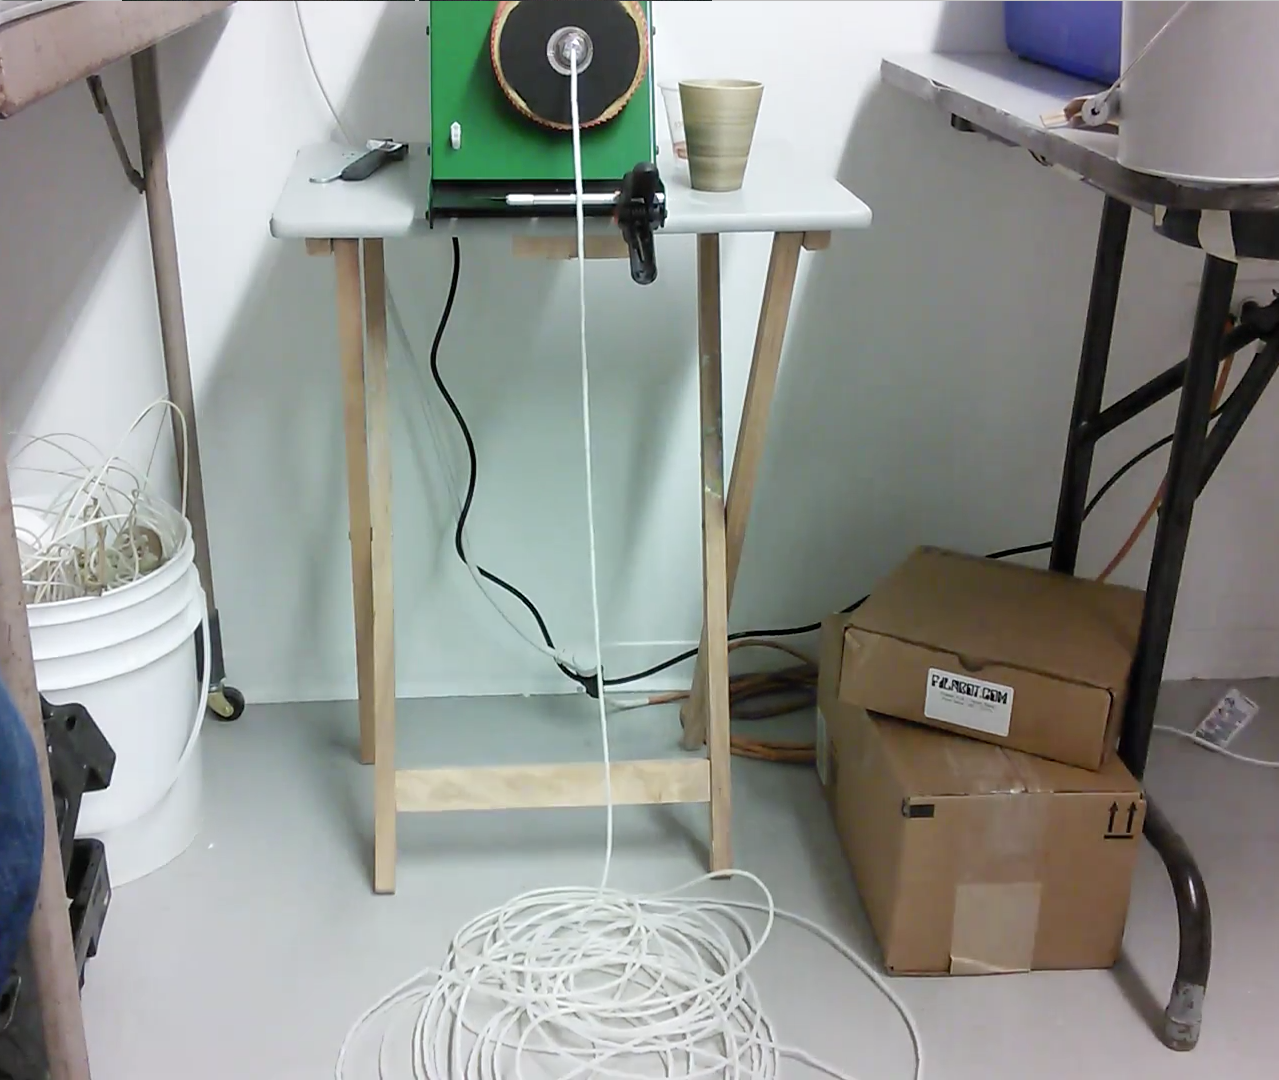
\includegraphics[width=\hsize]{art/extruding.png}
\caption{\label{fig:art_2} Extruding on a larger scale }
\end{figure}

\begin{figure}[h!]
\centering
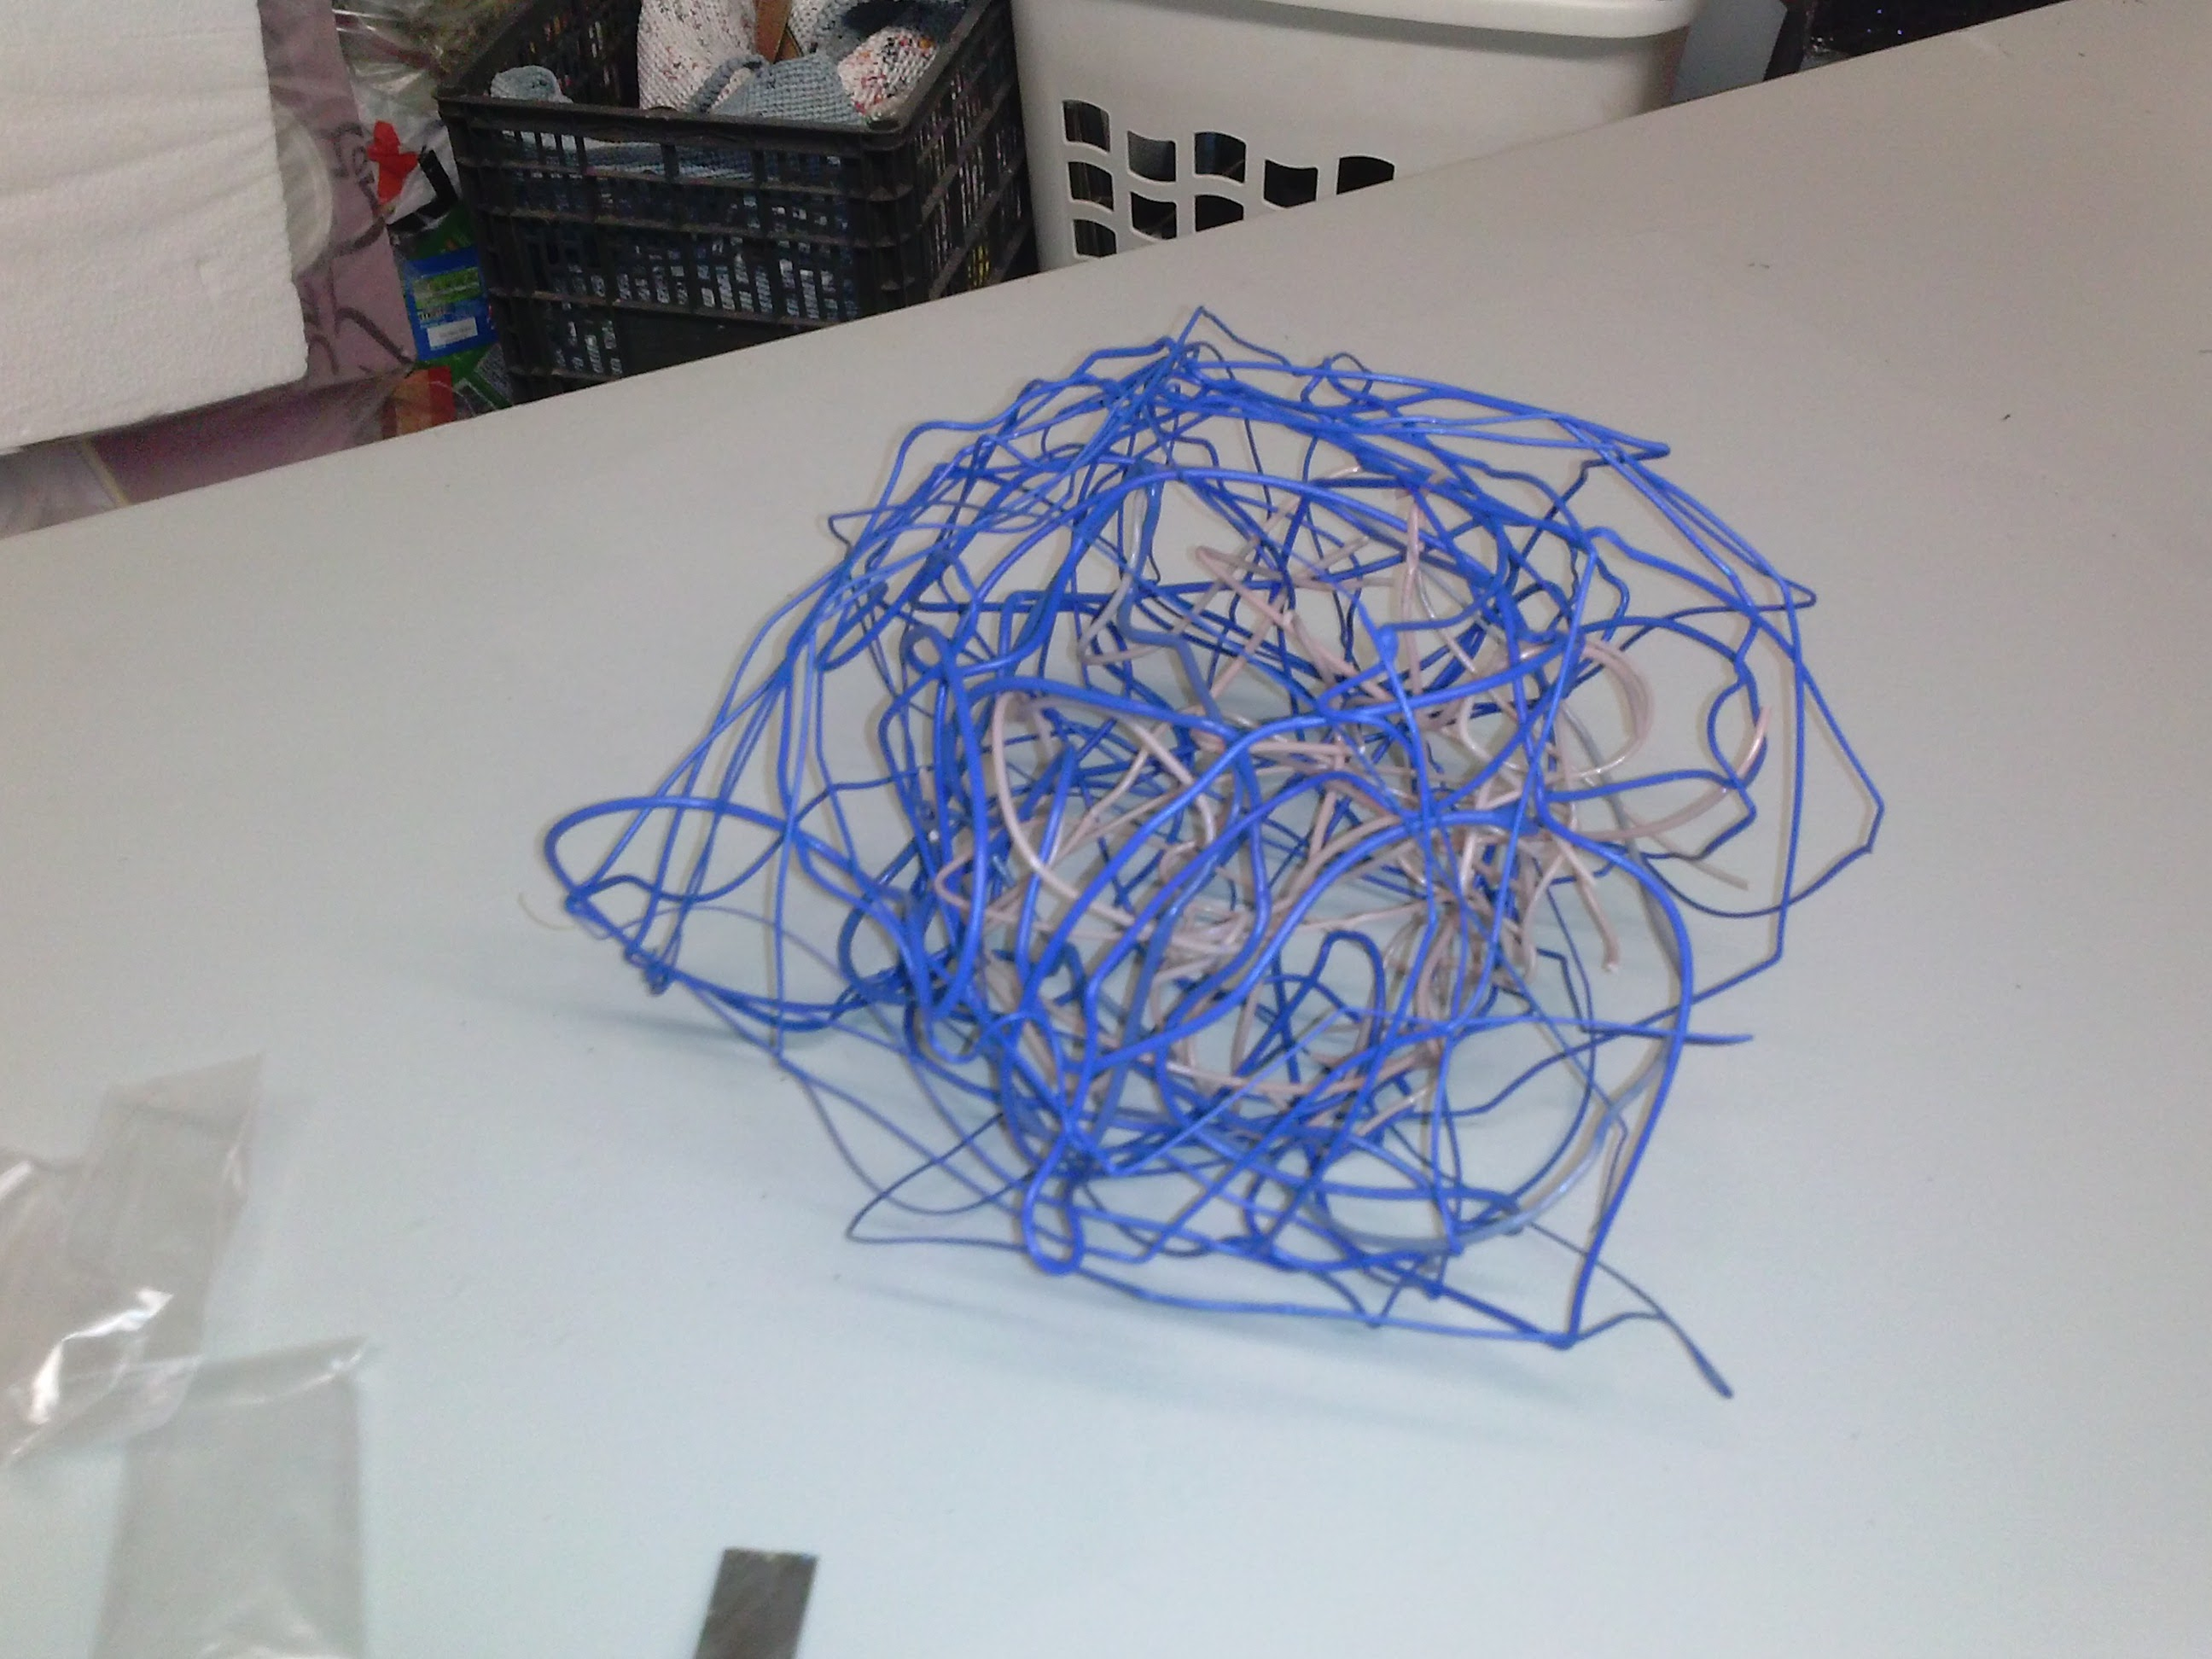
\includegraphics[width=\hsize]{art/CAM00454.jpg}
\caption{\label{fig:art_1} Larger scale sculpture }
\end{figure}



\begin{figure}[h!]
\centering
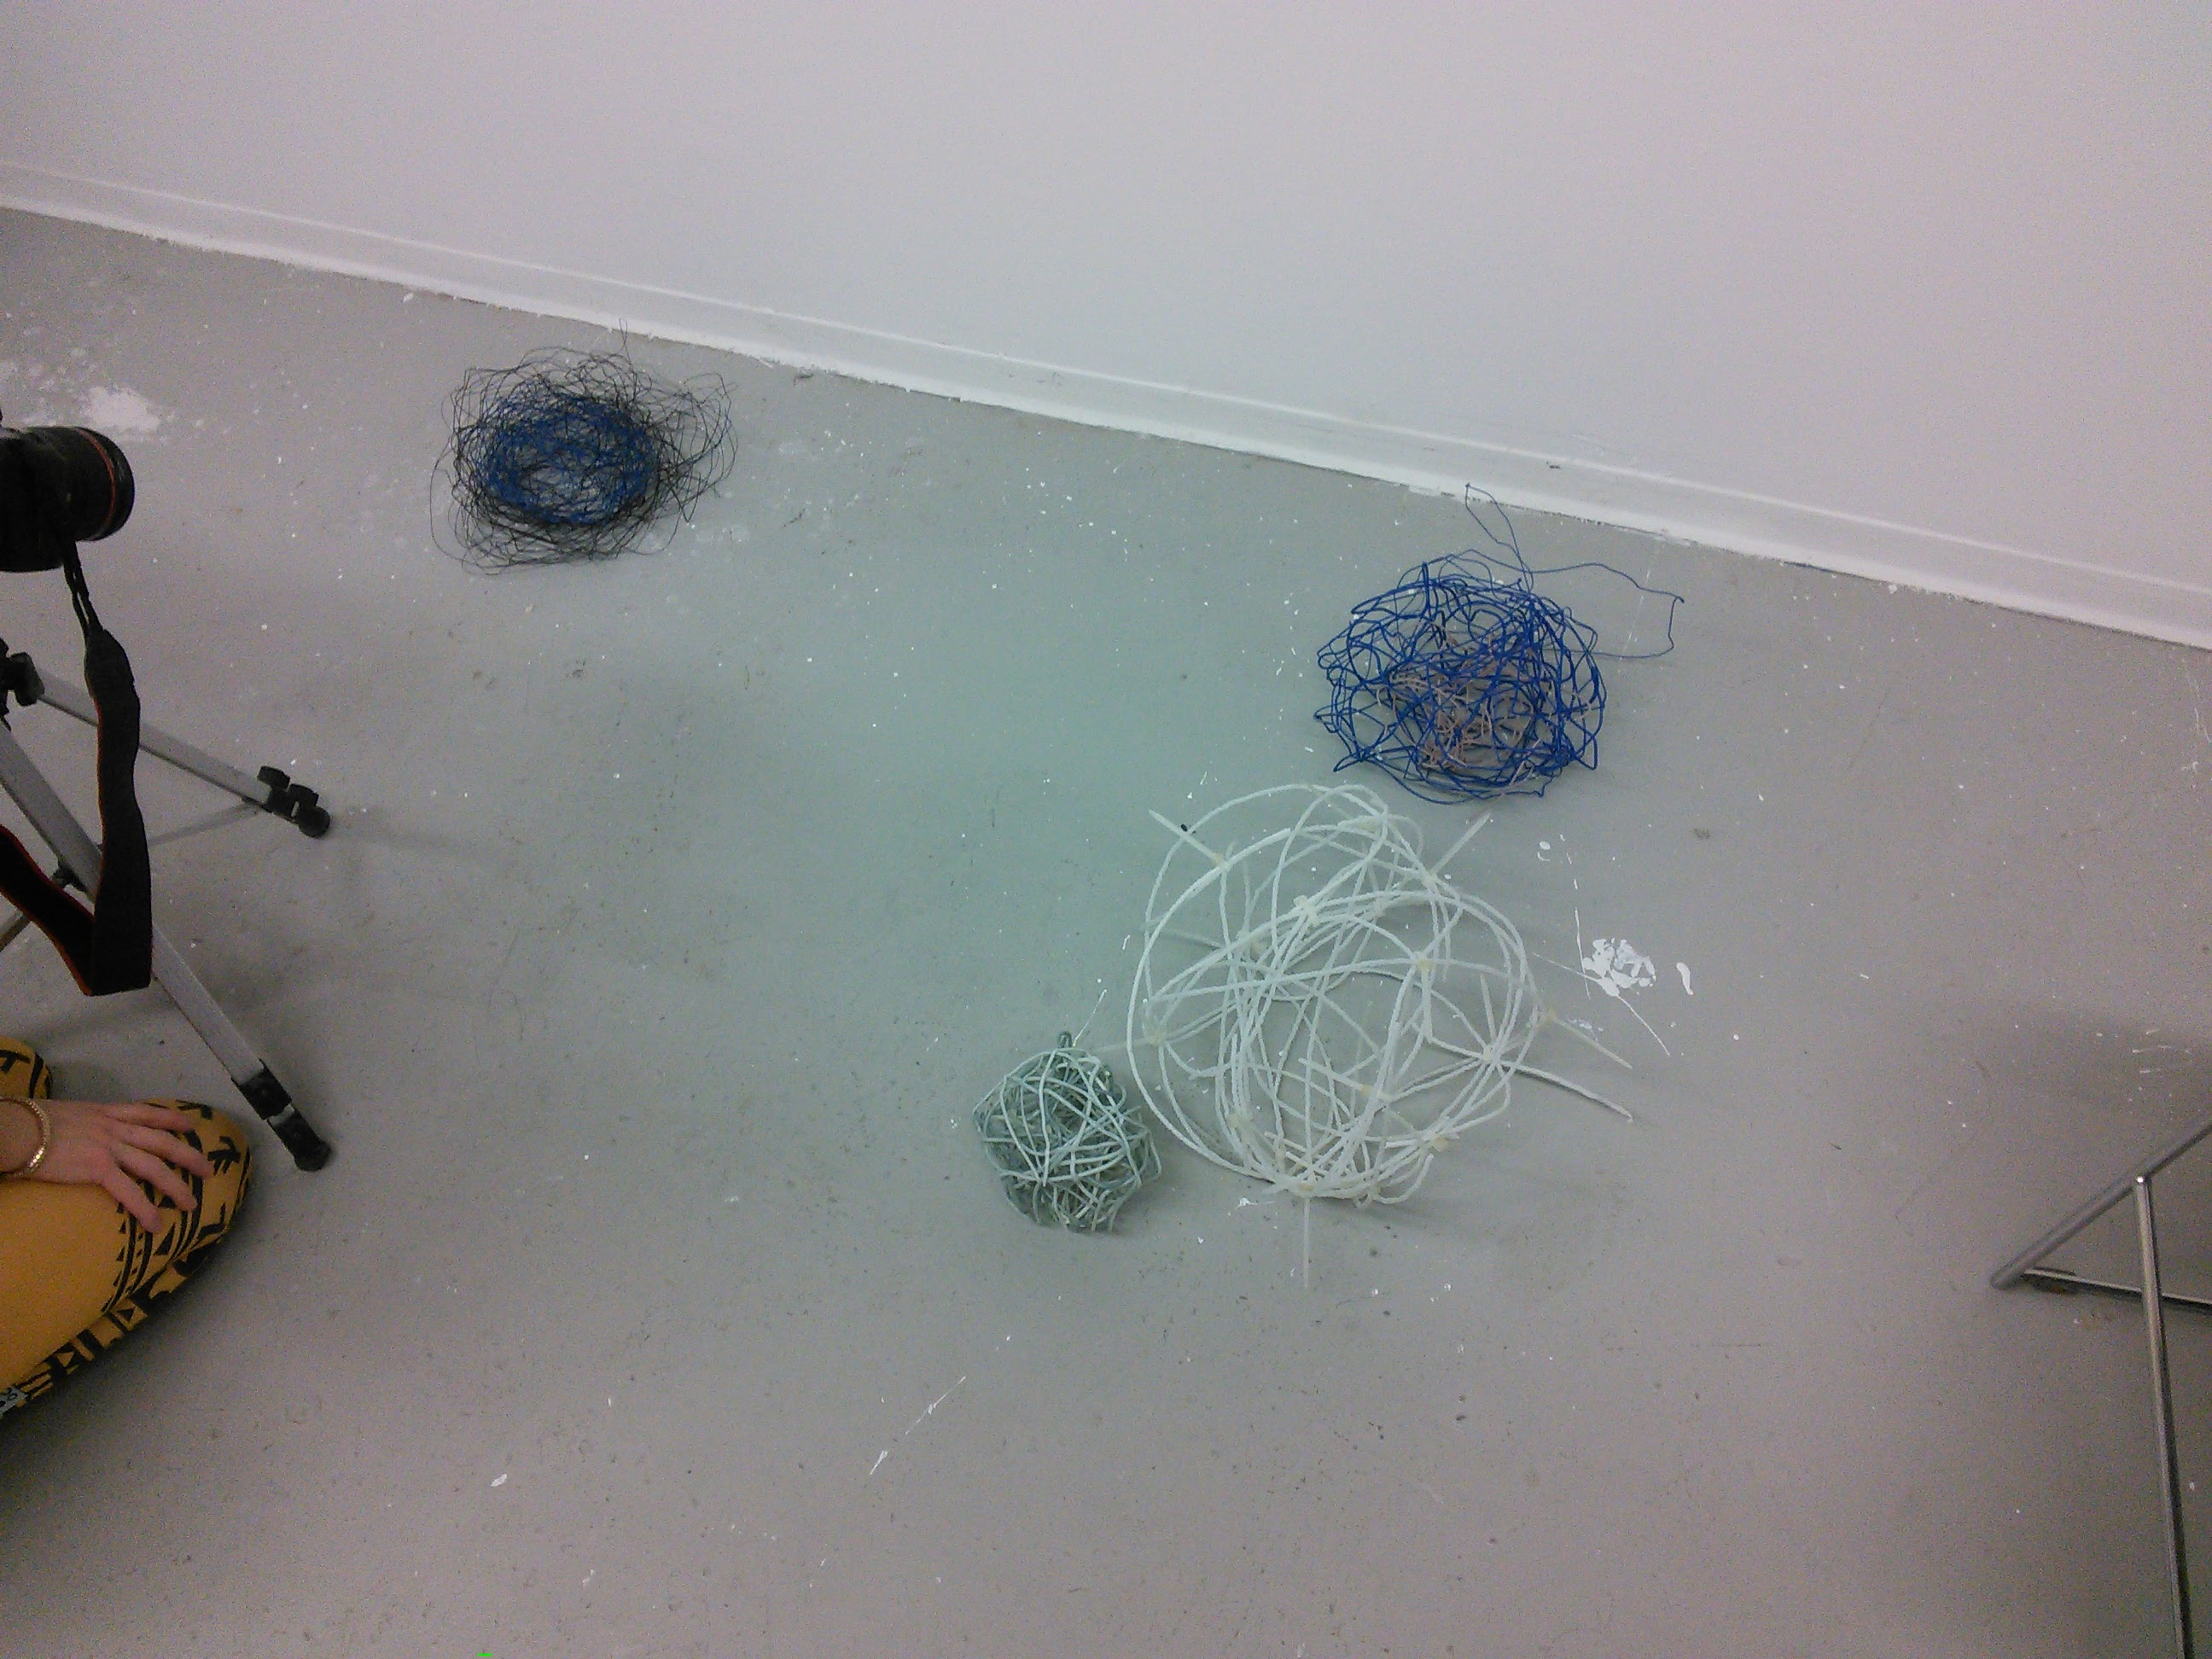
\includegraphics[width=\hsize]{art/IMG_20160205_113249.jpg}
\caption{\label{fig:art_3} Multiple larger sculptures }
\end{figure}